\documentclass[11pt,table]{beamer}
\mode<presentation>
\usepackage{etex}
\usepackage{graphicx}
\usepackage{epstopdf}
\usepackage[english]{babel}
\usepackage{tabularx}
\usepackage{booktabs}
\usepackage{mathrsfs}
\usepackage{multicol}
\usepackage{bm}
\usepackage{subcaption}
\usepackage{wrapfig}
\usepackage{dcolumn}
\usepackage{threeparttable}
\usepackage{booktabs}
\usepackage{bbm}
\usepackage{amsmath,dsfont,listings}
\usepackage{amssymb}
\usepackage{rotating}
\usepackage{multirow}
\usepackage[authoryear]{natbib}
\usepackage{circledsteps}
\usepackage{tikz}
\usetikzlibrary{arrows,decorations.pathmorphing,backgrounds,fit,positioning,shapes.symbols,chains}
\setbeamertemplate{section in toc}[sections numbered]
\setbeamertemplate{caption}[numbered]

\bibliographystyle{Econometrica}

\setbeamersize{text margin right=3.5mm, text margin left=7.5mm}  % text margin
\setbeamersize{sidebar width left=0cm, sidebar width right=0mm}
\setbeamertemplate{sidebar right}{}
\setbeamertemplate{sidebar left}{}

\definecolor{text-grey}{rgb}{0.45, 0.45, 0.45} % grey text on white background
\definecolor{bg-grey}{rgb}{0.66, 0.65, 0.60} % grey background (for white text)
\definecolor{fu-blue}{RGB}{0, 51, 102} % blue text
\definecolor{fu-green}{RGB}{153, 204, 0} % green text
\definecolor{fu-red}{RGB}{204, 0, 0} % red text (used by \alert)

\setbeamertemplate{frametitle}{%
    \vskip-30pt \color{text-grey}\large%
    \begin{minipage}[b][23pt]{80.5mm}%
    \flushleft\insertframetitle%
    \end{minipage}%
}

\setbeamertemplate{navigation symbols}{} 

%%% begin title page
\setbeamertemplate{title page}{
\vskip2pt\hfill
\vskip19pt\hskip3pt

% set the title and the author
\vskip4pt
\parbox[top][1.35cm][c]{11cm}{\LARGE\color{text-grey} Econome\textcolor{red1}{tricks}: \inserttitle \\[1ex] \small \quad \\[3ex]}
\vskip17pt
\parbox[top][1.35cm][c]{11cm}{\small Trick 01: \insertsubtitle \\[2ex] \insertauthor \\[1ex]}
%insert meta data
\tiny \textcolor{white}{\insertdate}\\
\textcolor{white}{Description:}\\
\textcolor{white}{This guide introduces basic concepts of probability theory.}

}
%%% end title page

%%% colors
\usecolortheme{lily}
\setbeamercolor*{normal text}{fg=black,bg=white}
\setbeamercolor*{alerted text}{fg=fu-red}
\setbeamercolor*{example text}{fg=fu-green}
\setbeamercolor*{structure}{fg=fu-blue}

\setbeamercolor*{block title}{fg=white,bg=black!50}
\setbeamercolor*{block title alerted}{fg=white,bg=black!50}
\setbeamercolor*{block title example}{fg=white,bg=black!50}

\setbeamercolor*{block body}{bg=black!10}
\setbeamercolor*{block body alerted}{bg=black!10}
\setbeamercolor*{block body example}{bg=black!10}

\setbeamercolor{bibliography entry author}{fg=fu-blue}
\setbeamercolor{bibliography entry journal}{fg=text-grey}
\setbeamercolor{item}{fg=fu-blue}
\setbeamercolor{navigation symbols}{fg=text-grey,bg=bg-grey}
%%% end colors

%%% headline
\setbeamertemplate{headline}{
\vskip30pt
}
%%% end headline

%%% footline
\newcommand{\footlinetext}{
%\insertshortinstitute, \insertshorttitle, \insertshortdate
}
\setbeamertemplate{footline}{
\vskip2pt
\hfill \raisebox{-1pt}{\usebeamertemplate***{navigation symbols}}
\hfill \insertframenumber\hspace{10pt}
\vskip4pt
}
%%% end footline

%%% settings for listings package
\lstset{extendedchars=true, showstringspaces=false, basicstyle=\footnotesize\sffamily, tabsize=2, breaklines=true, breakindent=10pt, frame=l, columns=fullflexible}
\lstset{language=Java} % this sets the syntax highlighting
\lstset{mathescape=true} % this switches on $...$ substitution in code
% enables UTF-8 in source code:
\lstset{literate={ä}{{\"a}}1 {ö}{{\"o}}1 {ü}{{\"u}}1 {Ä}{{\"A}}1 {Ö}{{\"O}}1 {Ü}{{\"U}}1 {ß}{\ss}1}
%%% end listings

\usepackage{concmath}
\usepackage{xcolor}
\definecolor{red1}{RGB}{206, 17, 38}
\definecolor{blue1}{RGB}{16, 118, 208}
\definecolor{gray1}{RGB}{117, 115, 115}
\usepackage{hyperref}


\newtheorem{proposition}{Proposition}
\newtheorem{assumption}{Definition}

\title[]{Short guides to econometrics}
\subtitle[]{Review of Probability Theory}
\author[D. Rostam-Afschar]{\textcolor{gray1}{Davud Rostam-Afschar (Uni Mannheim)}}
\date[]{\today}
\subject{Econometrics}
\renewcommand{\footlinetext}{\insertshortinstitute, \insertshorttitle, \insertshortdate}
\hypersetup{
    bookmarks=false,
    unicode=false,
    pdftoolbar=false,
    pdffitwindow=true,
    pdftitle={Short Guides to Econometrics: Probability Theory},
    pdfauthor={Davud Rostam-Afschar},
    pdfsubject={Probability Theory},
    pdfkeywords={probability theory, probability fundamentals, mean and variance, moments of a random variable, useful rules},
    pdfnewwindow=true,
}
\def\sym#1{\ifmmode^{#1}\else\(^{#1}\)\fi}

\begin{document}

\begin{frame}[plain]
  \titlepage
\end{frame}

% --------------------------------------------------- Slide --
\begin{frame}
	\frametitle{Content}
	\tableofcontents[]
\end{frame}

\section{Probability fundamentals}
\begin{frame}{Discrete and continuous random variables}
\begin{minipage}{0.5\linewidth}
\begin{itemize}
  \item A random variable $X$ is $\textbf{discrete}$ if the set of outcomes $x$ is either finite or countably
infinite.
  \item  The random variable $X$ is $\textbf{continuous}$ if the set of outcomes $x$ is infinitely divisible and, hence,
not countable.
\end{itemize}
\end{minipage}
\hspace{10pt}
\begin{minipage}{0.35\linewidth}\centering
{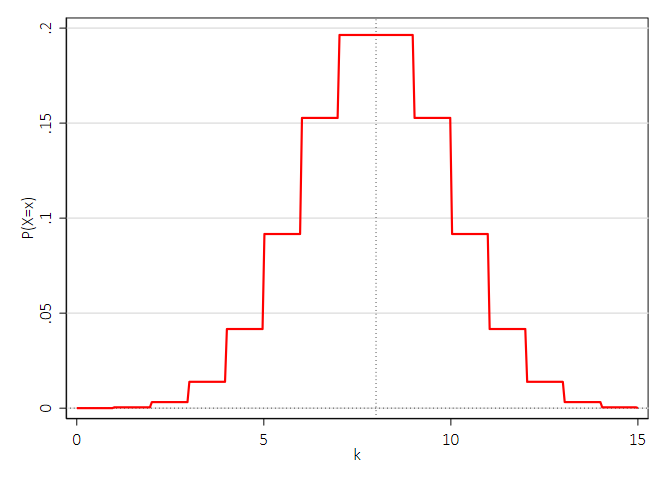
\includegraphics[width=1\textwidth]{figures/binomial_pdf}}
{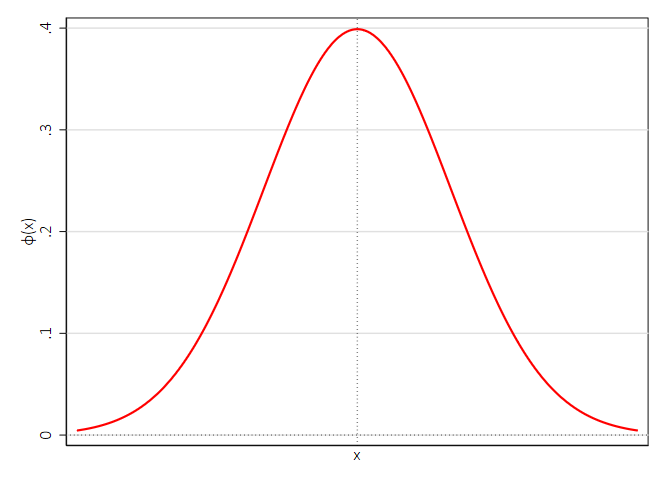
\includegraphics[width=1\textwidth]{figures/normal_pdf}}
\end{minipage}
\end{frame}

\begin{frame}{Discrete probabilities}
For values $x$ of a discrete random variable $X$,\\ the \textbf{probability mass function} (pmf)
$$f(x)=Prob(X=x).$$
The axioms of probability require
$$0\leq Prob(X=x)\leq1,$$
$$\sum_x f(x)=1.$$
\end{frame}

\begin{frame}{Discrete cumulative probabilities}
For values $x$ of a discrete random variable $X$,\\ the \textbf{cumulative distribution function}
$$F(x)=\sum_{X\leq x}f(x)=Prob(X\leq x),$$
where
$$f(x_i)=F(x_i)-F(x_{i-1}).$$
\begin{example} 
\scriptsize
\renewcommand{\baselinestretch}{1}
Roll of a six-sided die
\vspace{-5mm}

\renewcommand{\baselinestretch}{1}
	\begin{center}
		\begin{threeparttable}[htbp]

\label{tab:timeline}
\scriptsize
		\begin{tabular}{lll}
\toprule
$x$ & $f(x)$ & $F(X\leq x)$\\
\midrule
1 & $f(1)=1/6$ & $F(X\leq 1)=1/6$\\
2 & $f(2)=1/6$ & $F(X\leq 2)=2/6$\\
3 & $f(3)=1/6$ & $F(X\leq 3)=3/6$\\
4 & $f(4)=1/6$ & $F(X\leq 4)=4/6$\\
5 & $f(5)=1/6$ & $F(X\leq 5)=5/6$\\
6 & $f(6)=1/6$ & $F(X\leq 6)=6/6$\\
\bottomrule
		\end{tabular}

	\end{threeparttable}
\end{center}
\renewcommand{\baselinestretch}{1.45}
%-------------------------------------------
What's the probability that you roll a 5 or higher? $F(X\geq 5) = 1 - F(X\leq 4) = 1-2/3 = 1/3.$
\end{example}

\end{frame}

\begin{frame}{Continuous probabilities}
For values $x$ of a continuous random variable $X$, the probability is zero but the area under $f(x)\geq0$ in the range form $a$ to $b$ is\\ the \textbf{probability density function} (pdf)
$$Prob(a\leq x\leq b)=Prob(a< x< b)=\int_a^bf(x)dx\geq 0.$$
The axioms of probability require
$$\int^{+\infty}_{-\infty} f(x)dx=1.$$
$f(x)=0$ outside the range of $x$.\\
The \textbf{cumulative distribution function} (cdf) is
$$F(x)=\int_{-\infty}^x f(t)dt,$$
$$f(x)=\frac{dF(x)}{dx}.$$
\end{frame}

\begin{frame}{Cumulative distribution function}
For continuous and discrete variables, $F(x)$ satisfies
\small
\begin{assumption} \textbf{Properties of cdf}. 
\begin{itemize}
	\item $0\leq F(x)\leq 1$
	\item If $x>y$, then $F(x)\geq F(y)$
	\item $F(+\infty)=1$
	\item $F(-\infty)=0$
\end{itemize}
and $$Prob(a< x\leq b)=F(b)-F(a).$$
\end{assumption}

\end{frame}


\begin{frame}{Symmetric distributions}
For symmetric distributions $$f(\mu - x) = f(\mu + x)$$
and $$1-F(x)=F(-x).$$
\begin{figure}[H]
\begin{center}
%\scalebox{.36}
{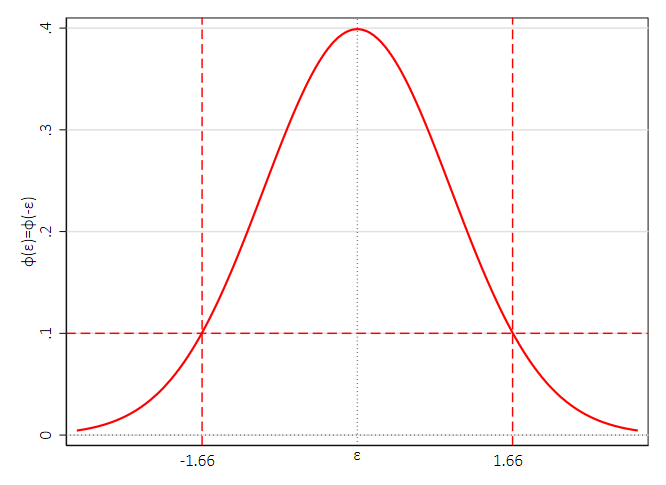
\includegraphics[height=0.45\textheight]{figures/normal_pdf_sym}}\label{normal_pdf_sym}
{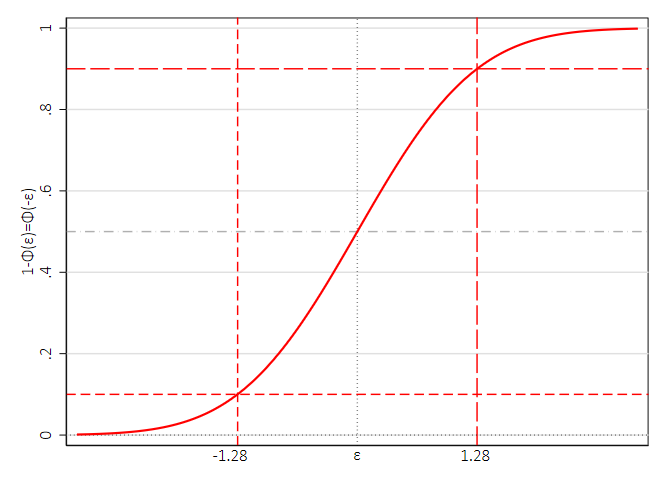
\includegraphics[height=0.45\textheight]{figures/normal_cdf_sym}}\label{normal_cdf_sym}
\end{center}
\end{figure}
\end{frame}

\section{Mean and variance}

\begin{frame}{Mean of a random variable}
The $\textbf{mean}$, or $\textbf{expected value}$, of a discrete random variable is
\begin{equation} \mu=E[x]=
\sum_{x}xf(x)
\end{equation}
\small
\begin{example} 
\scriptsize
\renewcommand{\baselinestretch}{1}
Roll of a six-sided die
\vspace{-5mm}
%-------------------------------------------
\renewcommand{\baselinestretch}{1}
	\begin{center}
		\begin{threeparttable}[htbp]
\label{tab:timeline}
\scriptsize
		\begin{tabular}{lll}
\toprule
$x$ & $f(x)=1/n$ & $F(X\leq x)=(x-a+1)/n$\\
\midrule
a = 1 & $f(1)=1/6$ & $F(X\leq 1)=1/6$\\
2 & $f(2)=1/6$ & $F(X\leq 2)=2/6$\\
3 & $f(3)=1/6$ & $F(X\leq 3)=3/6$\\
4 & $f(4)=1/6$ & $F(X\leq 4)=4/6$\\
5 & $f(5)=1/6$ & $F(X\leq 5)=5/6$\\
b = 6 & $f(6)=1/6$ & $F(X\leq 6)=6/6$\\
\bottomrule
		\end{tabular}
	\end{threeparttable}
\end{center}
\renewcommand{\baselinestretch}{1.45}
%-------------------------------------------
What's the expected value from rolling the dice? $E[x]=1/6+2/6+3/6+4/6+5/6+6/6=3.5.$\\
This is the mean (and the median) of a uniform distribution $(n+1)/2=(a+b)/2=3.5$.\\
\end{example}
\end{frame}


\begin{frame}{Mean of a random variable}

For a continuous random variable $x$, the expected value is $$E[x]={\int_{x}xf(x)dx.}$$

\begin{example} 
\scriptsize
\renewcommand{\baselinestretch}{1}
The continuous uniform distribution is $1/(b-a)$ for $a\leq x\leq b$ and $0$ otherwise.\\

$$E[x]={\int_{a}^b\frac{x}{b-a}dx}={\frac{1}{b-a}\int_{a}^bxdx}.$$

Antiderivative of $x$ is $x^2/2$
$$E[x]={\frac{1}{b-a} b^2/2-a^2/2}=\frac{(b-a)(b+a)}{2(b-a)}=\frac{a+b}{2}.$$


The mean (and the median) is again $(a+b)/2=3.5$.
\end{example}
\scriptsize
For a function $g(x)$ of $x$, the expected value is $E[g(x)]=\sum_{x}g(x) Prob(X = x)$ or $E[g(x)]=\int_{x}g(x)f(x)dx$. If $g(x) = a + bx$ for constants $a$ and $b$, then $E[a + bx] = a + bE[x]$.
\end{frame}



\begin{frame}{Variance of a random variable}
The $\textbf{variance}$ of a random variable $\sigma^{2}>0$ is
\begin{equation}\label{eq0} \sigma^2=Var[x] = E[(x - \mu)^{2}]=\left\{
 \begin{array}{ll}
 {\sum_{x}(x - \mu)^{2}f(x)~~~~if~ x~ is~ discrete, } \\
 {~}\\
 {\int_{x}(x - \mu)^{2}f(x)dx~~if~ x~ is~ continuous.}
 \end{array}
 \right.
\end{equation}
\begin{example} 
\scriptsize
\renewcommand{\baselinestretch}{1}
Roll of a six-sided die. What's the variance $V[x]$ from rolling the dice?\\
The probability of observing $x$, $Pr(X=x)=1/n$, is discretely uniformly distributed
$$E[x]=\frac{n+1}{2}; \; (E[x])^2=\frac{(n+1)^2}{4}.$$
$$E[x^2]=\sum_xPr(X=x)=\frac{1}{n}\sum_{x=1}^nx^2=\frac{(n+1)(2n+1)}{6} \text{ due to the sequence sum of squares}.$$
$$V[x] = E[x^{2}] - (E[x])^2.$$
 $V[x]=\frac{(n+1)(2n+1)}{6}-\frac{(n+1)^2}{4}=\frac{n^2-1}{12}=(6^2-1)/12\approx2.92.$\\
\end{example}

\end{frame}



\begin{frame}{Chebychev inequality}

For any random variable $x$ and any positive constant $k$,
$$\Pr(\mu - k\sigma \leq x \leq \mu + k\sigma) \geq \frac{1}{k^{2}}.$$
\footnotesize
\textbf{Share outside $k$ standard deviations}.\\
If $x$ is normally distributed, the bound is $1-(2\Phi(k)-1)$.
\begin{figure}[H]
\begin{center}
%\scalebox{.36}
{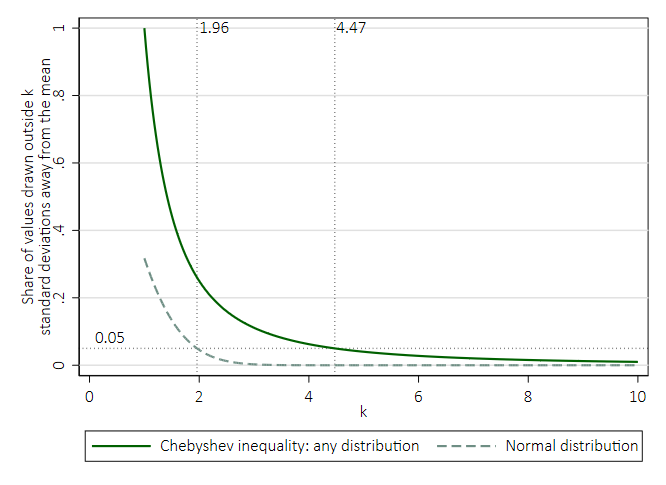
\includegraphics[height=0.55\textheight]{figures/chebyshev_inequality_pdf}}\label{chebyshev_inequality_pdf}
\end{center}
\end{figure}
95\% of the observations are within 1.96 standard deviations for normally distributed $x$. If $x$ is not normal, 95\% are at most within 4.47 standard deviations.

\end{frame}


\begin{frame}{Normal coverage}
\begin{figure}
	\centering
		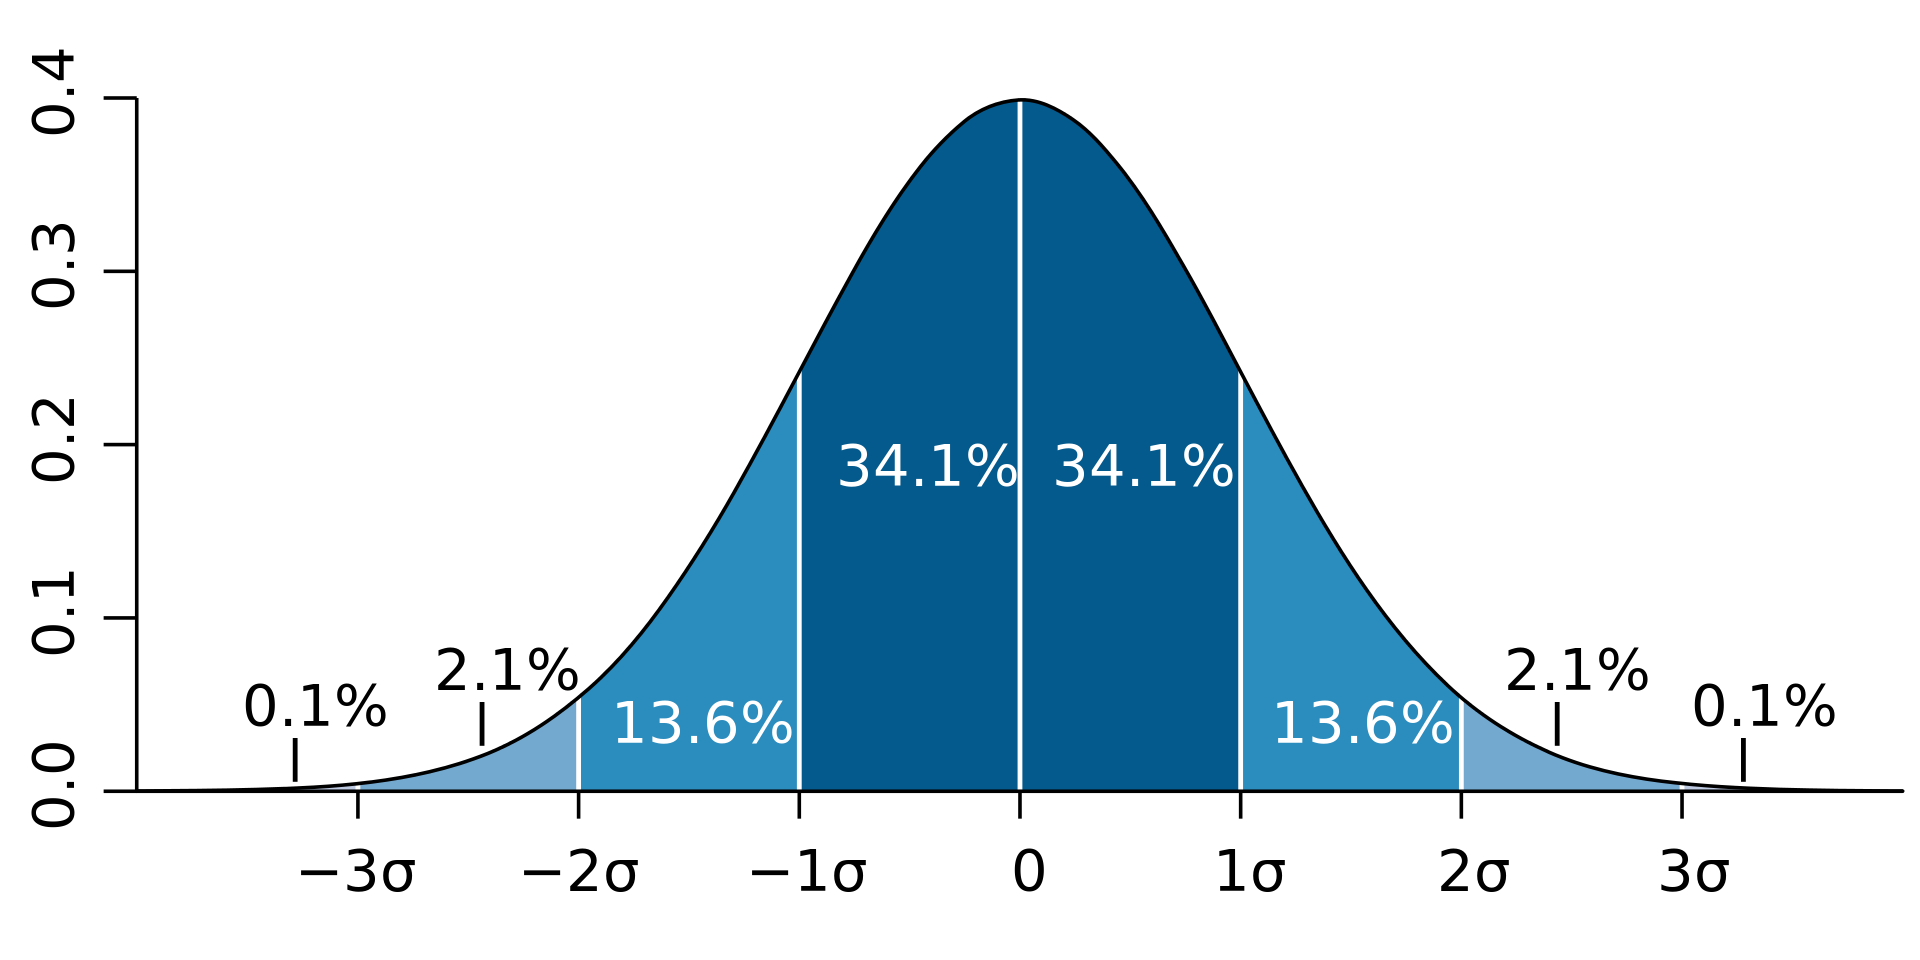
\includegraphics[width=0.70\textwidth]{figures/Standard_deviation_diagram.png}
	\label{fig:Standard_deviation_diagram}
\end{figure}

\end{frame}

\section{Moments of a random variable}

\begin{frame}{Central moments of a random variable}
The central moments are
 \begin{equation*}
    \mu_{r} = E[(x - \mu)^{r}].
 \end{equation*}
\small
\begin{example} \textbf{Moments}. 
Two measures often used to describe a probability distribution are
\begin{itemize}
	\item expectation $= E[(x - \mu)^{1}]$
	\item variance $= E[(x - \mu)^{2}]$
	\item skewness $= E[(x - \mu)^{3}]$
	\item kurtosis $= E[(x - \mu)^{4}]$
\end{itemize}
The skewness is zero for symmetric distributions.
\end{example}

\end{frame}

\begin{frame}{Higher order moments}
\begin{figure}[H]
\begin{center}
{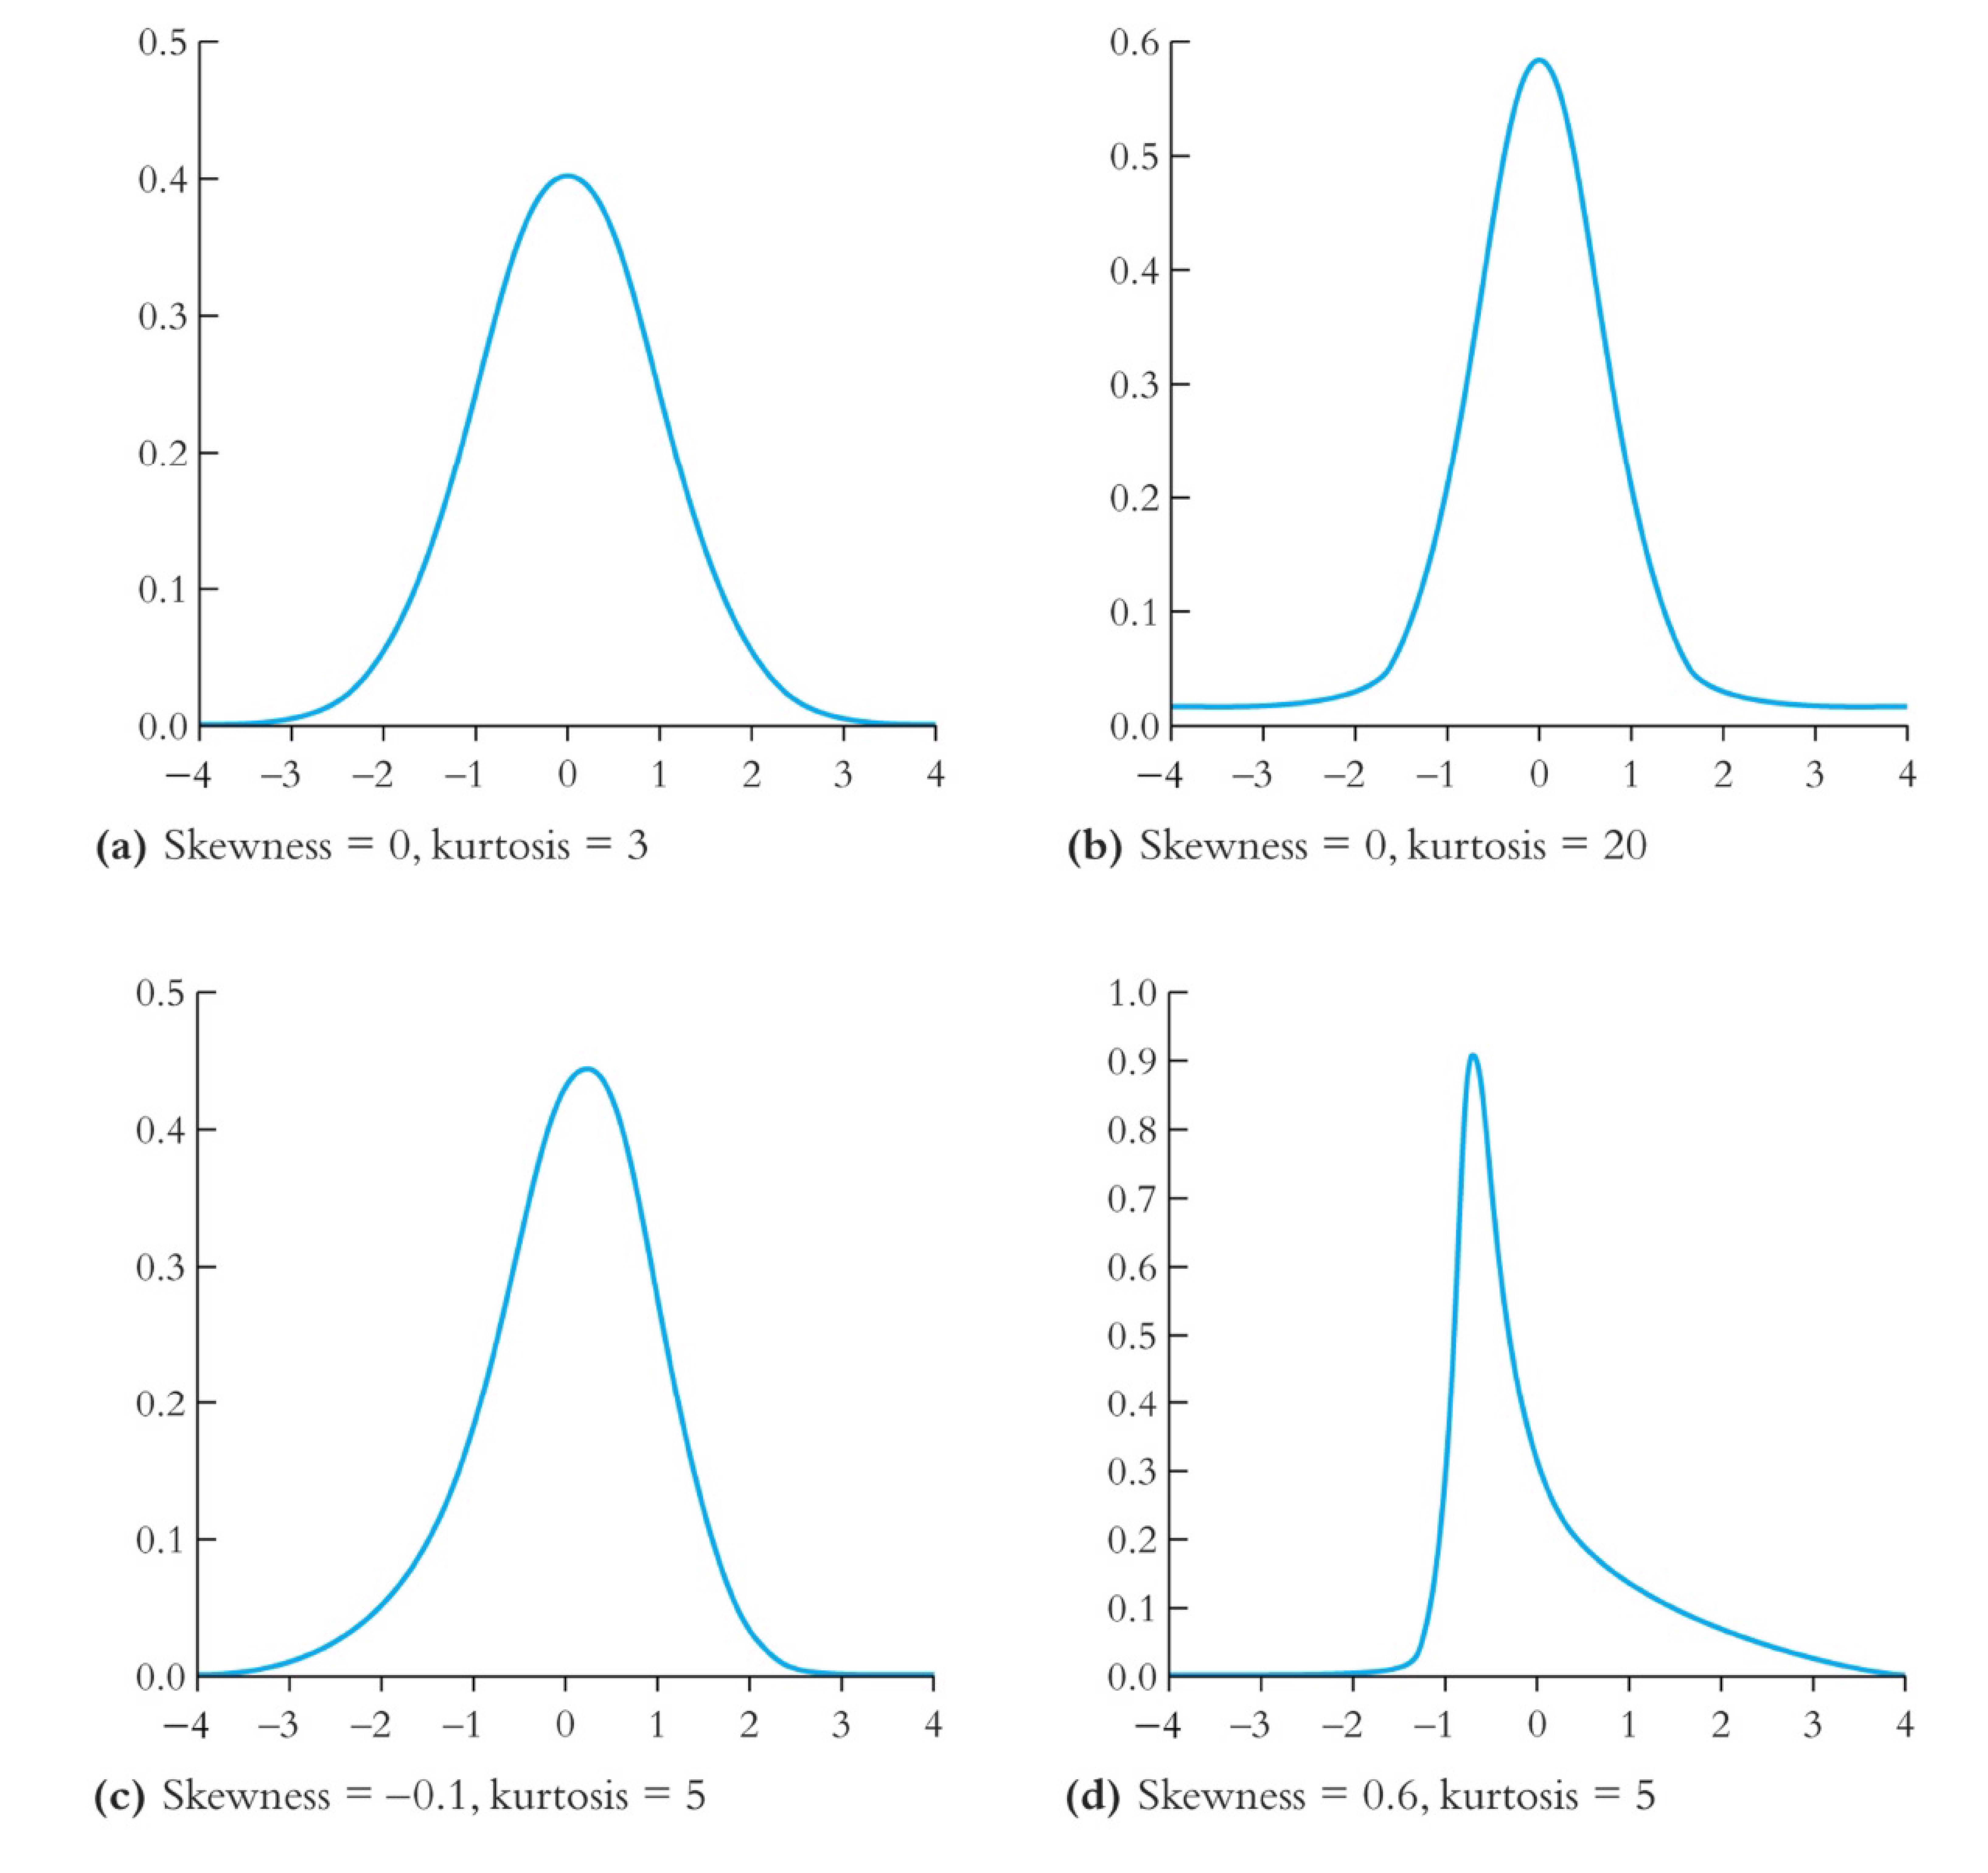
\includegraphics[width=0.7\textwidth]{figures/skewness_kurtosis}}\label{skewness_kurtosis}
\end{center}
\end{figure}
\end{frame}

\begin{frame}{Moment generating function}
For the random variable $X$, with probability density function $f(x)$, if the function
\begin{equation*}
    M(t) = E[e^{tx}].
\end{equation*}
exists, then it is the $\textbf{moment generating function}(MGF)$.

\begin{itemize}
	\item Often simpler alternative to working directly with probability density functions or cumulative distribution functions
	\item Not all random variables have moment-generating functions
\end{itemize}
The $n$th moment is the $n$th derivative of the moment-generating function, evaluated at $t=0$. 

\begin{example}
The MGF for the standard normal distribution with $\mu=0, \sigma=1$ is $$M_{z}(t) = e^{\mu t+ \sigma^2t^{2}/2} = e^{t^{2}/2}.$$
If $x$ and $y$ are independent, then the MGF of $x + y$ is $M_{x}(t)M_{y}(t).$
\end{example}
\end{frame}


\begin{frame}{Moment generating function}
\small
For $x \sim N (\mu, \sigma^2)$ for some $\mu,\sigma>0$ with moment generating function ${M_x}'(t) =  \exp (\mu t + \dfrac 1 2 \sigma^2 t^2)$, the first moment generating function of $x$ is
$$ E[(x - \mu)^{1}]={M_x}'(t)= (\mu +  \sigma^2 t)\exp \bigg(\mu t + \dfrac 1 2 \sigma^2 t^2\bigg).$$
\small
\begin{example}
$$ E[(x - \mu)^{1}]={M_x}'(t) = \frac{d\bigg[\exp \bigg(\mu t + \dfrac 1 2 \sigma^2 t^2\bigg)\bigg]}{dt}$$ 
$$= \frac{d\bigg[\mu t + \dfrac 1 2 \sigma^2 t^2\bigg]}{dt}\frac{d\bigg[\exp \bigg(\mu t + \dfrac 1 2 \sigma^2 t^2\bigg)\bigg]}{d(\mu t + \dfrac 1 2 \sigma^2 t^2)}$$
$$ =(\mu +  \sigma^2 t)\exp \bigg(\mu t + \dfrac 1 2 \sigma^2 t^2\bigg).$$
\end{example}
\end{frame}


\begin{frame}{Moment generating function}
\small
If $x\sim N(0,1)$, 
\begin{itemize}
	\item the skewness is $E[(x - \mu)^{3}]=0$ and
	\item the kurtosis is $E[(x - \mu)^{4}]=3$.
\end{itemize}
\scriptsize
\begin{example}
\vspace{-5mm}
$$E[(x - \mu)^{1}]={M_x}'(t) =(\mu +  \sigma^2 t)\exp \bigg(\mu t + \dfrac 1 2 \sigma^2 t^2\bigg) \text{ with } \mu=0, \sigma=1, t=0: E[x]=\mu=0$$
$$E[(x - \mu)^{2}]={M_x}''(t) =  \bigg(\sigma^2 + (\mu + \sigma^2 t)^2 \bigg)  \exp \bigg(\mu t + \dfrac 1 2 \sigma^2 t^2\bigg)$$ $$\text{ with } \mu=0, \sigma=1, t=0: E[(x - \mu)^{2}]=\sigma^2=1$$
$$E[(x - \mu)^{3}]={M_x}'''(t) =\bigg(3 \sigma^2 (\mu + \sigma^2 t) + (\mu + \sigma^2 t)^3\bigg)  \exp\bigg(\mu t + \dfrac 1 2 \sigma^2 t^2\bigg)$$
$$\text{with } \mu=0, \sigma=1, t=0: E[(x - \mu)^{3}]= 0$$
$$E[(x - \mu)^{4}]={M_x}^{(4)} (t) = \bigg(3 \sigma^4 + 6 \sigma^2 (\mu + \sigma^2 t)^2 + (\mu + \sigma^2 t)^4\bigg) \exp\bigg(\mu t + \dfrac 1 2 \sigma^2 t^2\bigg)$$
$$\text{with } \mu=0, \sigma=1, t=0: E[(x - \mu)^{4}]=3.$$
\end{example}
\end{frame}

\begin{frame}{Approximating mean and variance}
For any two functions $g_{1}(x)$ and $g_{2}(x)$,
 \begin{equation}
    E[g_{1}(x) + g_{2}(x)] = E[g_{1}(x)] + E[g_{2}(x)].
 \end{equation}
 For the general case of a possibly nonlinear $g(x)$,
 {\begin{equation}
    E[g(x)] =\int_{x}g(x)f(x)dx,
 \end{equation}
 and
 \begin{equation}
    Var[g(x)] =\int_{x}\left(g(x) - E [g(x)]\right)^{2}f(x)dx.
 \end{equation}}
$E[g(x)]$ and $Var[g(x)]$ can be approximated by a first order linear Taylor series:
\begin{equation}\label{eq5}
    g(x)\approx [g(x^{0})-g^{\prime}(x^{0})x^{0}]+g^{\prime}(x^{0})x.
\end{equation}
\end{frame}


\begin{frame}{Taylor approximation Order 1}
\begin{figure}
	\centering
		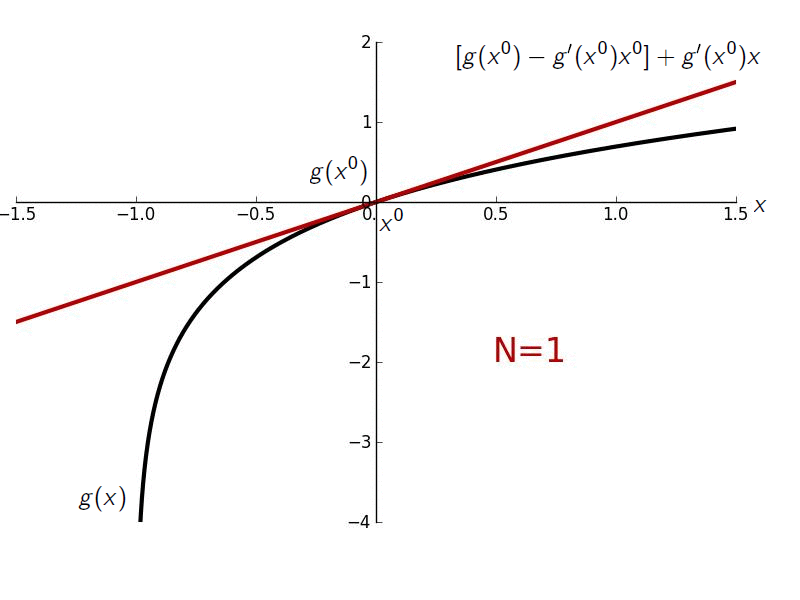
\includegraphics[width=0.90\textwidth]{figures/taylor1_formula.png}
	\label{fig:taylor1_formula}
\end{figure}
\tiny Thanks to Shiyu Chang
\end{frame}

%
%\begin{frame}{Taylor approximation Order 1}
%\begin{figure}
	%\centering
		%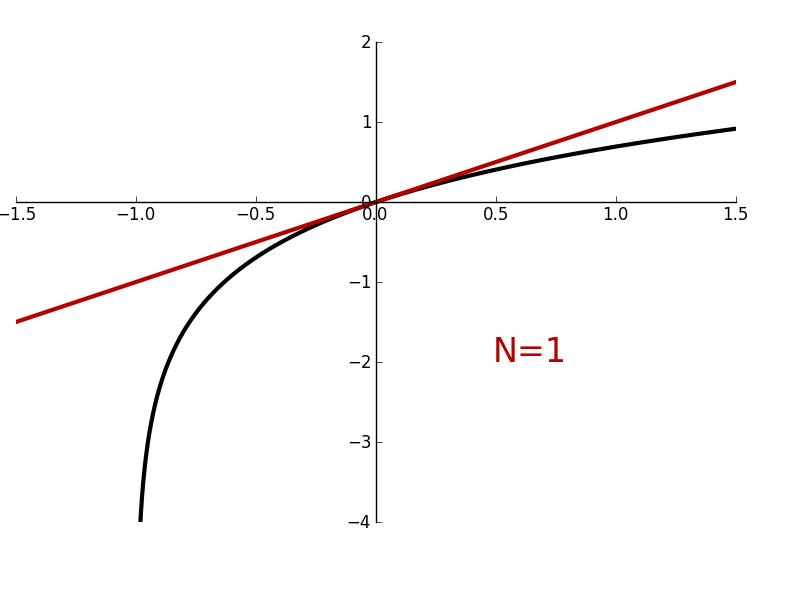
\includegraphics[width=0.90\textwidth]{taylor1.png}
	%\label{fig:taylor1}
%\end{figure}
%
%\end{frame}
%
%\begin{frame}{Taylor approximation Order 2}
%\begin{figure}
	%\centering
		%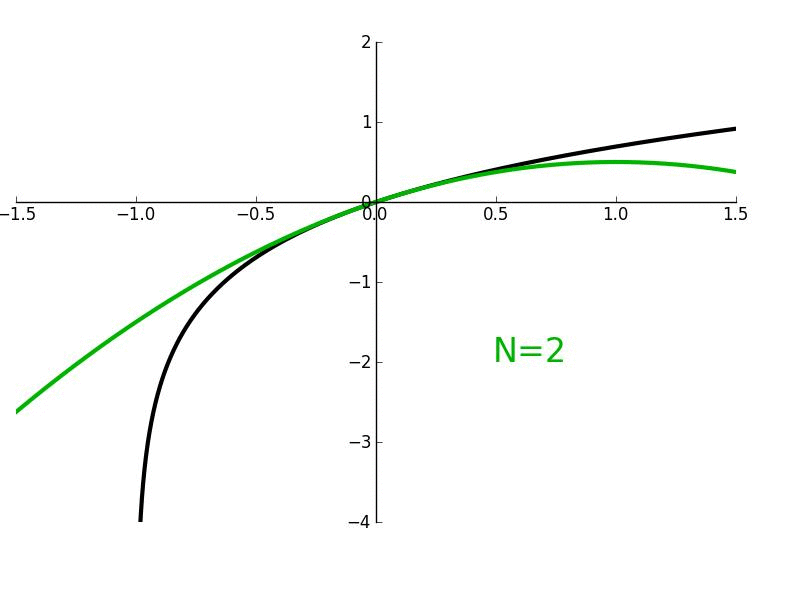
\includegraphics[width=0.90\textwidth]{taylor2.png}
	%\label{fig:taylor2}
%\end{figure}
%
%\end{frame}
%
%
%\begin{frame}{Taylor approximation Order 3}
%\begin{figure}
	%\centering
		%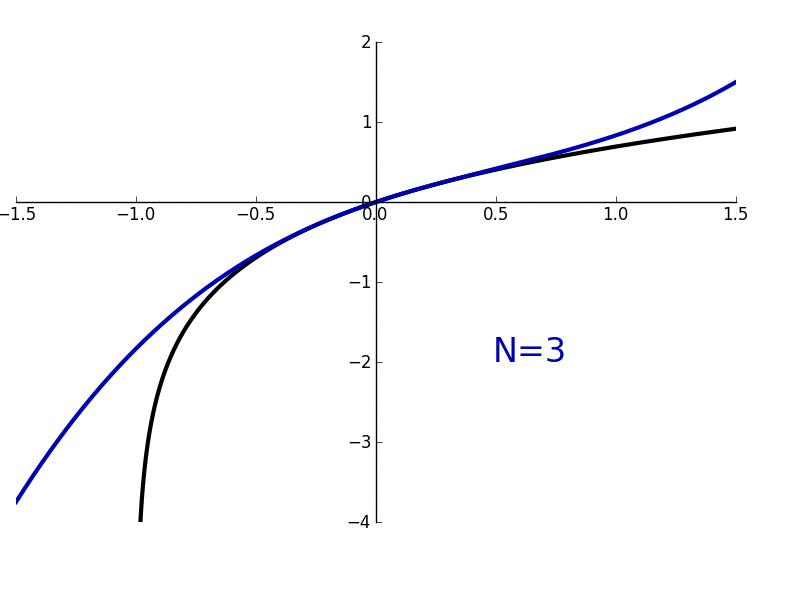
\includegraphics[width=0.90\textwidth]{taylor3.png}
	%\label{fig:taylor3}
%\end{figure}
%
%\end{frame}
%
%\begin{frame}{Taylor approximation Order 4}
%\begin{figure}
	%\centering
		%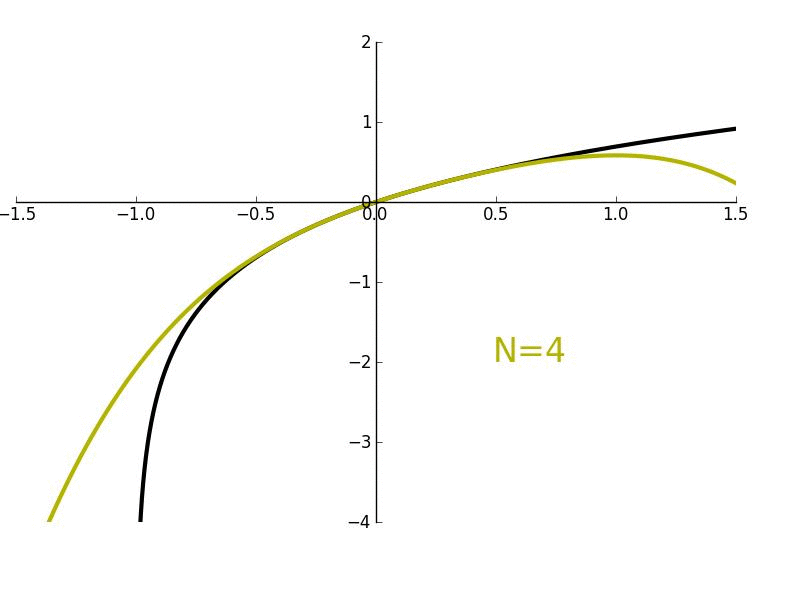
\includegraphics[width=0.90\textwidth]{taylor4.png}
	%\label{fig:taylor4}
%\end{figure}
%
%\end{frame}
%
%\begin{frame}{Taylor approximation Order 5}
%\begin{figure}
	%\centering
		%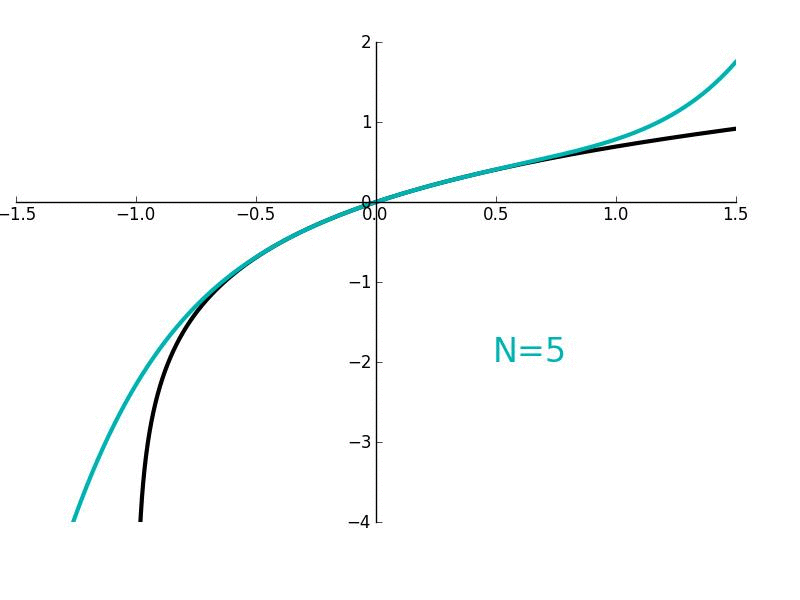
\includegraphics[width=0.90\textwidth]{taylor5.png}
	%\label{fig:taylor5}
%\end{figure}
%
%\end{frame}
%
%\begin{frame}{Taylor approximation Order 6}
%\begin{figure}
	%\centering
		%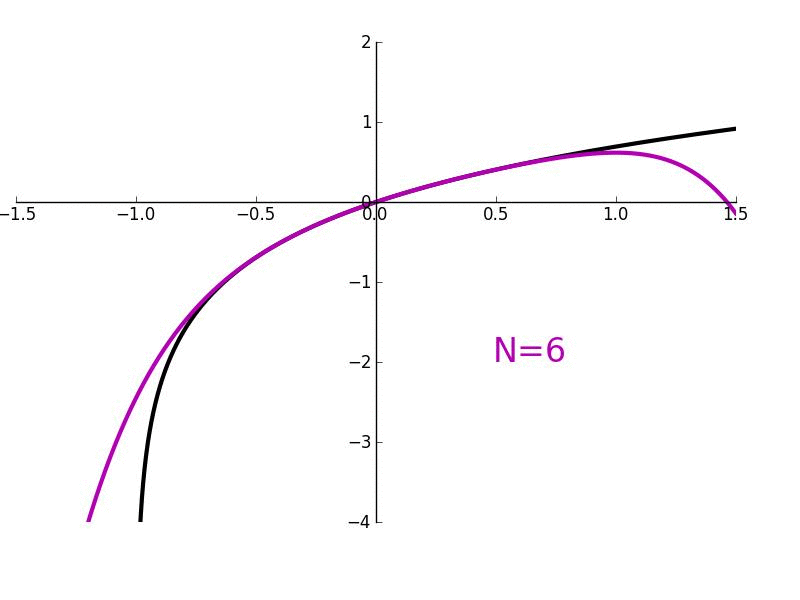
\includegraphics[width=0.90\textwidth]{taylor6.png}
	%\label{fig:taylor6}
%\end{figure}
%
%\end{frame}
%
%\begin{frame}{Taylor approximation Order 7}
%\begin{figure}
	%\centering
		%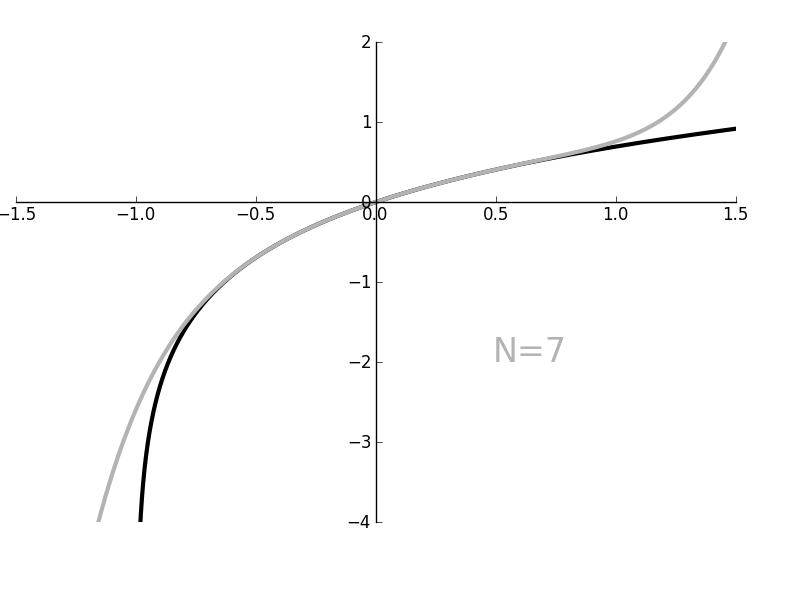
\includegraphics[width=0.90\textwidth]{taylor7.png}
	%\label{fig:taylor7}
%\end{figure}
%
%\end{frame}
%
%\begin{frame}{Taylor approximation Order 8}
%\begin{figure}
	%\centering
		%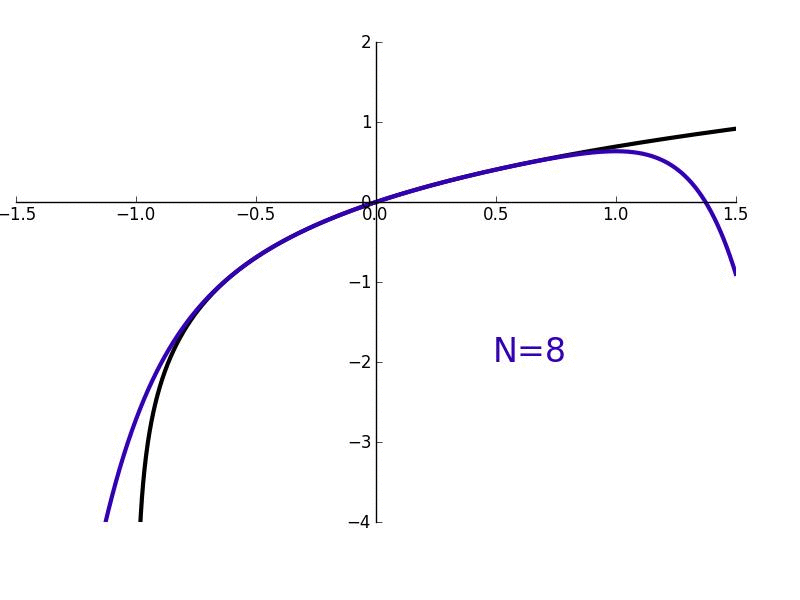
\includegraphics[width=0.90\textwidth]{taylor8.png}
	%\label{fig:taylor8}
%\end{figure}
%
%\end{frame}
%
%\begin{frame}{Taylor approximation Order 9}
%\begin{figure}
	%\centering
		%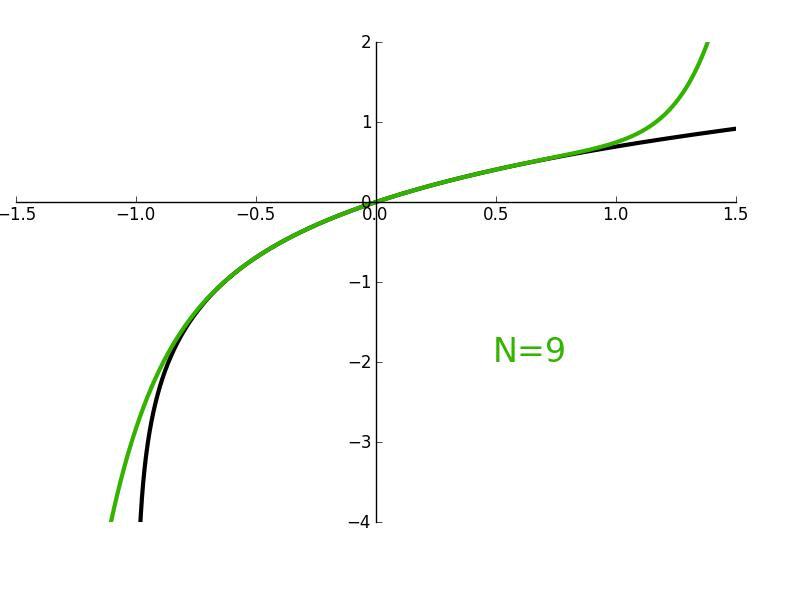
\includegraphics[width=0.90\textwidth]{taylor9.png}
	%\label{fig:taylor9}
%\end{figure}
%
%\end{frame}
%
%\begin{frame}{Taylor approximation Order 10}
%\begin{figure}
	%\centering
		%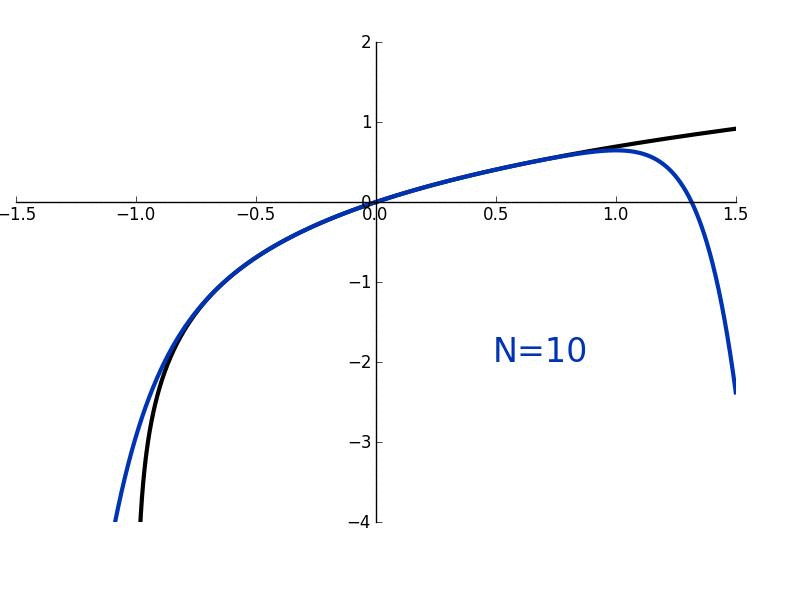
\includegraphics[width=0.90\textwidth]{taylor10.png}
	%\label{fig:taylor10}
%\end{figure}
%
%\end{frame}
%
%\begin{frame}{Taylor approximation Order 15}
%\begin{figure}
	%\centering
		%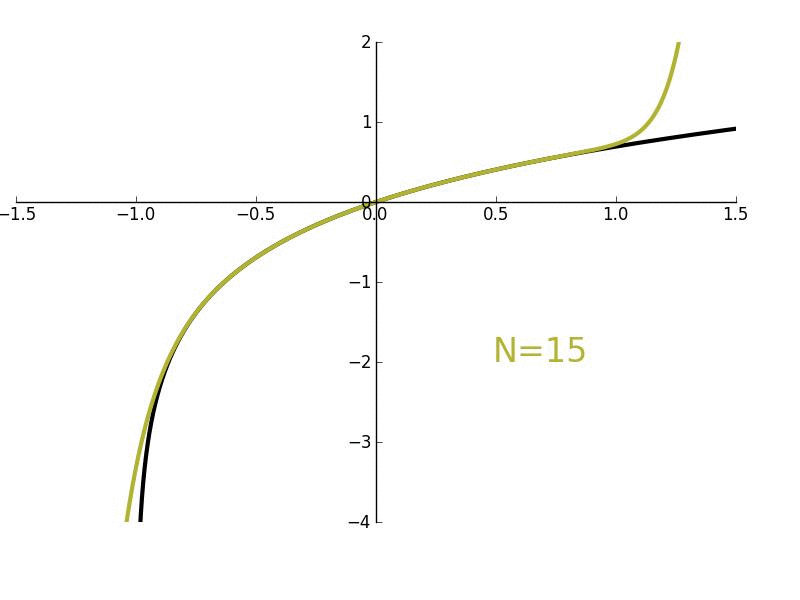
\includegraphics[width=0.90\textwidth]{taylor15.png}
	%\label{fig:taylor15}
%\end{figure}
%
%\end{frame}
%
%\begin{frame}{Taylor approximation Order 20}
%\begin{figure}
	%\centering
		%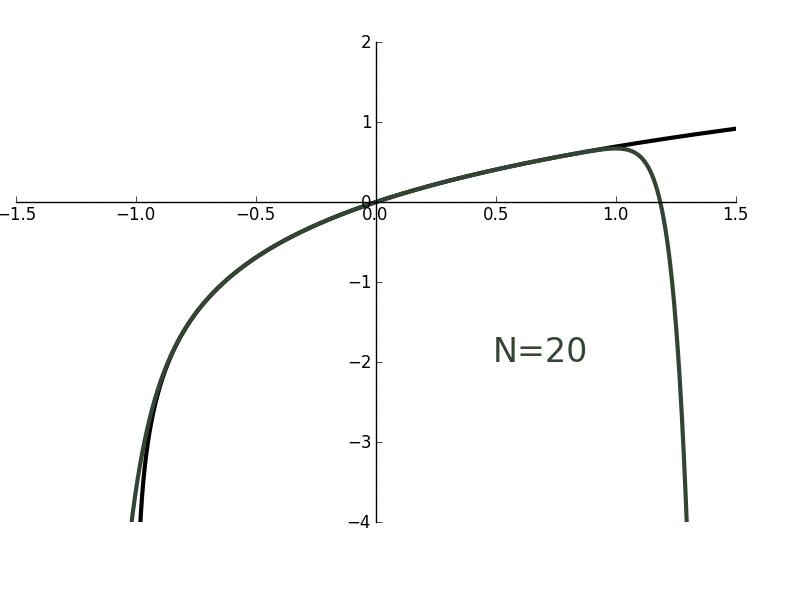
\includegraphics[width=0.90\textwidth]{taylor20.png}
	%\label{fig:taylor20}
%\end{figure}
%
%\end{frame}
%
%\begin{frame}{Taylor approximation Order 45}
%\begin{figure}
	%\centering
		%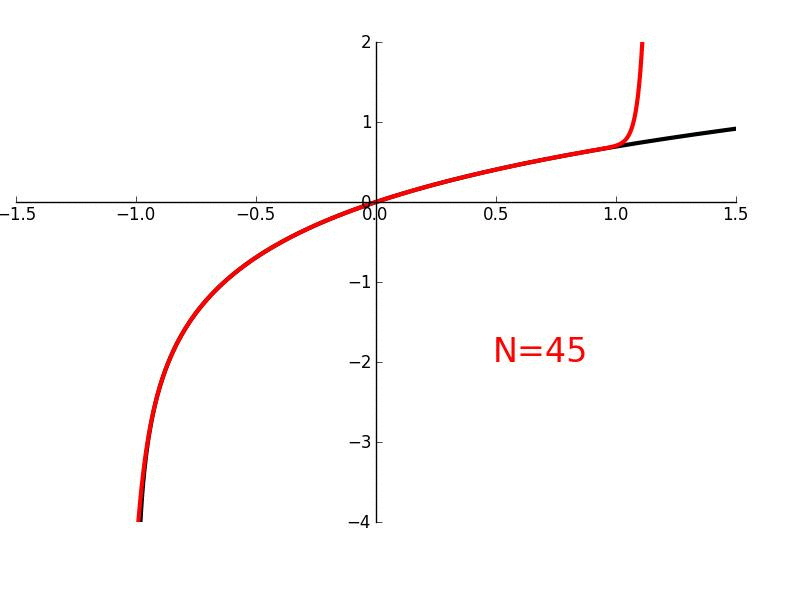
\includegraphics[width=0.90\textwidth]{taylor45.png}
	%\label{fig:taylor45}
%\end{figure}
%
%\end{frame}
%
%
%\begin{frame}{Taylor approximation Order 100}
%\begin{figure}
	%\centering
		%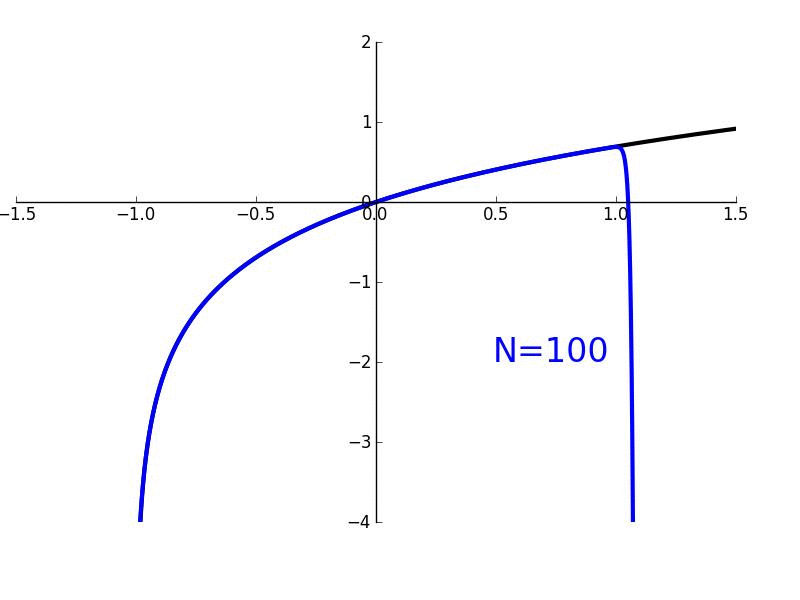
\includegraphics[width=0.90\textwidth]{taylor100.png}
	%\label{fig:taylor100}
%\end{figure}
%
%\end{frame}

\begin{frame}{Approximating mean and variance}

A natural choice for the expansion point is $x^{0} = \mu = E(x)$. Inserting this value in Eq. (\ref{eq5}) gives
\begin{equation}\label{eq6}
    g(x)\approx [g(\mu)-g^{\prime}(\mu)\mu]+g^{\prime}(\mu)x,
\end{equation}
so that
\begin{equation}\label{eq7}
    E[g(x)] \approx g(\mu),
\end{equation}
and
\begin{equation}\label{eq8}
    Var[g(x)]\approx [g^{\prime}(\mu)]^{2} Var[x].
\end{equation}
\scriptsize
\begin{example} \textbf{Isoelastic utility}.
$c_{bad}=$	10.00 Euro; $c_{good}=$	100.00 Euro;  probability good outcome	50\%\\[2ex]
$\mu=E[c]=1/2 \times c_{bad}+ 1/2 \times c_{good}=$55.00 Euro\\
$$u(c)= c^{1/2}$$
$u(\mu)= 7.42$ approximates $E[u(c)]= 1/2\times10^{1/2}+1/2\times100^{1/2}=6.58$
\end{example}

\end{frame}


\begin{frame}{Approximating mean and variance}

\small

\begin{example} \textbf{Isoelastic utility}.
\footnotesize
$c_{bad}=$	10.00 Euro; $c_{good}=$	100.00 Euro;  probability good outcome	50\%; $\mu=55.00$ Euro\\[2ex]

\begin{wrapfigure}{r}{0.5\textwidth}
  \vspace{-20pt}
  \begin{center}
		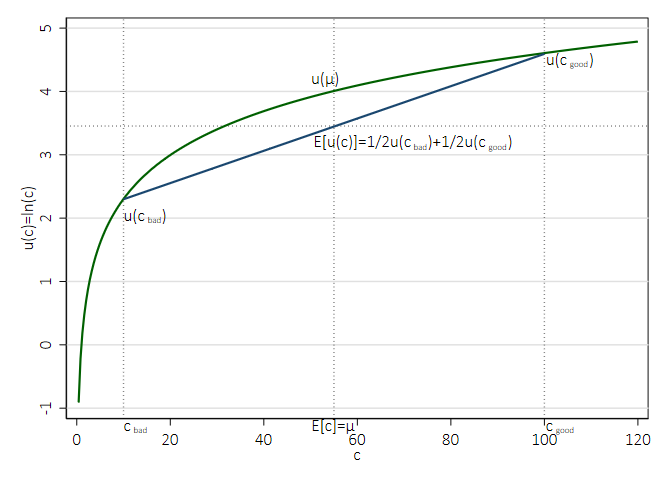
\includegraphics[height=0.46\textheight]{figures/Jensens_inequality.png}
	\label{fig:Jensens_inequality}
  \vspace{-40pt}
  \end{center}
\end{wrapfigure}

$$u(c)= \ln(c)$$
$u(\mu)= 4.01$ approx. $E[u(c)]= 1/2\times \ln(10)+1/2\times \ln(100)=3.45$\\[8ex]

\textbf{Jensen's inequality}: $E[g(x)]\leq g(E[x])]$ if $g''(x)<0$.\\[10ex]

$V[u(c)]\approx (1/55)^{2}((10-55)^2+(100-55)^2) =1.34$\\
$V[u(c)]= (\ln(10)-E[u(c)])^2+(\ln(100)-E[u(c)])^2 =2.65$
\end{example}

\end{frame}

\section{Useful rules}

\begin{frame}{Useful rules}
\renewcommand{\baselinestretch}{1.45}

\begin{itemize}
	\item $Var[x] = E[x^{2}] - \mu^{2}$
	\item $E[x^{2}] = \sigma^{2} + \mu^{2}$
	\item If $a$ and $b$ constants, $Var[a + bx] = b^{2} Var[x]$
	\item $Var[a] = 0$
	\item If $g(x) = a + bx$ and $a$ and $b$ are constants, $E[a + bx] = a + bE[x]$
	\item Coverage $\Pr(|X-\mu|\geq k\sigma) \leq \frac{1}{k^2}$
	\item Skewness $= E[(x - \mu)^{3}]$
	\item Kurtosis $= E[(x - \mu)^{4}]$
	\item For symmetric distributions $f(\mu - x) = f(\mu + x)$; $1-F(x)=F(-x)$
	\item $E[g(x)] \approx g(\mu)$
	\item $Var[g(x)]\approx [g^{\prime}(\mu)]^{2} Var[x]$
\end{itemize}
\renewcommand{\baselinestretch}{1}

\end{frame}

\begin{frame}[t,allowframebreaks
]\nocite{*}
\frametitle{References}
\small
\bibliography{bib}
\end{frame}


\end{document}
